
%\documentclass[journal]{IEEEtran}
\documentclass[journal,9pt]{igtesymp}
% *** GRAPHICS RELATED PACKAGES ***
%
\ifCLASSINFOpdf
  % \usepackage[pdftex]{graphicx}
  % declare the path(s) where your graphic files are
  % \graphicspath{{../pdf/}{../jpeg/}}
  % and their extensions so you won't have to specify these with
  % every instance of \includegraphics
  % \DeclareGraphicsExtensions{.pdf,.jpeg,.png}
\else
  % or other class option (dvipsone, dvipdf, if not using dvips). graphicx
  % will default to the driver specified in the system graphics.cfg if no
  % driver is specified.
  % \usepackage[dvips]{graphicx}
  % declare the path(s) where your graphic files are
  % \graphicspath{{../eps/}}
  % and their extensions so you won't have to specify these with
  % every instance of \includegraphics
  % \DeclareGraphicsExtensions{.eps}
\fi
% graphicx was written by David Carlisle and Sebastian Rahtz. It is
% required if you want graphics, photos, etc. graphicx.sty is already
% installed on most LaTeX systems. The latest version and documentation can
% be obtained at: 
% http://www.ctan.org/tex-archive/macros/latex/required/graphics/
% Another good source of documentation is "Using Imported Graphics in
% LaTeX2e" by Keith Reckdahl which can be found as epslatex.ps or
% epslatex.pdf at: http://www.ctan.org/tex-archive/info/
%
% latex, and pdflatex in dvi mode, support graphics in encapsulated
% postscript (.eps) format. pdflatex in pdf mode supports graphics
% in .pdf, .jpeg, .png and .mps (metapost) formats. Users should ensure
% that all non-photo figures use a vector format (.eps, .pdf, .mps) and
% not a bitmapped formats (.jpeg, .png). IEEE frowns on bitmapped formats
% which can result in "jaggedy"/blurry rendering of lines and letters as
% well as large increases in file sizes.
%
% You can find documentation about the pdfTeX application at:
% http://www.tug.org/applications/pdftex


% *** SUBFIGURE PACKAGES ***
\usepackage[tight,footnotesize]{subfigure}
% subfigure.sty was written by Steven Douglas Cochran. This package makes it
% easy to put subfigures in your figures. e.g., "Figure 1a and 1b". For IEEE
% work, it is a good idea to load it with the tight package option to reduce
% the amount of white space around the subfigures. subfigure.sty is already
% installed on most LaTeX systems. The latest version and documentation can
% be obtained at:
% http://www.ctan.org/tex-archive/obsolete/macros/latex/contrib/subfigure/
% subfigure.sty has been superceeded by subfig.sty.



\usepackage{graphicx}
%\usepackage{german}
%\usepackage{umlaute}


% *** Do not adjust lengths that control margins, column widths, etc. ***
% *** Do not use packages that alter fonts (such as pslatex).         ***
% There should be no need to do such things with IEEEtran.cls V1.6 and later.
% (Unless specifically asked to do so by the journal or conference you plan
% to submit to, of course. )



% correct bad hyphenation here
\hyphenation{op-tical net-works semi-conduc-tor}


\begin{document}
%
% paper title
% can use linebreaks \\ within to get better formatting as desired
\title{Unified Cauer Ladder + Surface Impedance Network \\
       via Turning-Point Basis Switch}
%
\author{K.~Sugahara\IEEEauthorrefmark{1},  H.~Nagamine\IEEEauthorrefmark{2},
and Y.~Hane\IEEEauthorrefmark{3}
 \\ \vspace{0.3cm} \normalsize{
\IEEEauthorblockA{\IEEEauthorrefmark{1}Faculty of Science and Engineering, Kindai University, 3-4-1 Kowakae, Higashi-Osaka, Osaka 577-8502, Japan\\
 \IEEEauthorrefmark{2}Faculty of Engineering, Gifu University, 1-1 Yanagido, Gifu 501-1193, Japan\\
 \IEEEauthorrefmark{3}Faculty of Science and Engineering, Toyo University, Kawagoe, Saitama, Japan\\
 E-mail: ksugahar@kindai.ac.jp}}%
}


% note the % following the last \IEEEmembership and also \thanks - 
% these prevent an unwanted space from occurring between the last author name
% and the end of the author line. i.e., if you had this:
% 
% \author{....lastname \thanks{...} \thanks{...} }
%                     ^------------^------------^----Do not want these spaces!
%
% a space would be appended to the last name and could cause every name on that
% line to be shifted left slightly. This is one of those "LaTeX things". For
% instance, "\textbf{A} \textbf{B}" will typeset as "A B" not "AB". To get
% "AB" then you have to do: "\textbf{A}\textbf{B}"
% \thanks is no different in this regard, so shield the last } of each \thanks
% that ends a line with a % and do not let a space in before the next \thanks.
% Spaces after \IEEEmembership other than the last one are OK (and needed) as
% you are supposed to have spaces between the names. For what it is worth,
% this is a minor point as most people would not even notice if the said evil
% space somehow managed to creep in.




% use for special paper notices
%\IEEEspecialpapernotice{(Invited Paper)}




\IEEEaftertitletext{\vspace{-1cm}\noindent\begin{abstract}
A truncated Cauer Ladder Network (CLN) is seamed to a Surface Impedance Boundary Condition (SIBC) element ($\alpha\!=\!1/2$ Constant Phase Element) at a turning point $\omega_N$ given by Matsuo's corner-frequency formula, with the SIBC scaling fixed by continuity (no fitting).  Formally this is the $s_\infty$ expansion point of the multiple-expansion-points CLN framework.  Analytical verification on a Cu slab reproduces the Stoll/Wall closed form across nine decades with ten Cauer rungs and one SIBC element; on a 3D Cu cuboid, an mpmath single-element VIM with HDiv divergence-free hex basis and an NGSolve HCurl Tanimoto-AT extraction yield matching unified $Y(j\omega)$ from two-to-three bulk Cauer rungs plus the SIBC element, cross-validated against a direct frequency-domain AC sweep.
\end{abstract}
\noindent\begin{keywords}
Cauer Ladder Network, Surface Impedance, Turning Point, Expansion Points, Eddy Current.
\end{keywords}\vspace{\baselineskip}}


\maketitle
\thispagestyle{empty}\pagestyle{empty}





% For peer review papers, you can put extra information on the cover
% page as needed:
% \ifCLASSOPTIONpeerreview
% \begin{center} \bfseries EDICS Category: 3-BBND \end{center}
% \fi
%
% For peerreview papers, this IEEEtran command inserts a page break and
% creates the second title. It will be ignored for other modes.
\IEEEpeerreviewmaketitle

\section{Unified CLN + SIBC}

A truncated Cauer Ladder Network (CLN) \cite{Kameari_2018} represents the eddy-current admittance $Y(s)\!=\!1/Z(s)$ as a continued fraction with rungs $(R_{2k},L_{2k+1})$ encoding the Foster eddy-mode spectrum.  The reliable rung count is bounded both by Hankel-Pad\'e ill-conditioning ($\!\sim\!300\times$ noise amplification per stage \cite{Nagamine_2026}) and, more fundamentally, by the basis's spatial resolution -- once skin depth $\delta(\omega)\!=\!\sqrt{2/(\omega\mu\sigma)}$ drops below the basis length scale, further rungs are non-physical.  In that regime, however, the Surface Impedance Boundary Condition $Z_s(j\omega)\!=\!\sqrt{j\omega\mu/\sigma}$ -- a Constant Phase Element of exponent $\alpha\!=\!1/2$ -- becomes exact.

We seam the two representations at a turning point $\omega_N$ given by Matsuo's corner-frequency formula \cite{Matsuo_2026} evaluated at the last reliable rung,
\begin{equation}
\omega_N \!=\! \sqrt{2^{\alpha/2}\!-\!1}\,R_{2N\!-\!2}/L_{2N\!-\!1} \!\approx\! 0.4350\,R_{2N\!-\!2}/L_{2N\!-\!1}, \label{eq:omegaN}
\end{equation}
yielding $Y_{\text{unified}}(j\omega)\!=\!1/Z_{\text{Cauer}}^{(N)}(j\omega)$ for $\omega\!<\!\omega_N$ and $K_{\text{SIBC}}\sqrt{\sigma/(j\omega\mu)}$ above, with $K_{\text{SIBC}}\!=\!Y_{\text{Cauer}}^{(N)}(j\omega_N)/\sqrt{\sigma/(j\omega_N\mu)}$ fixed by continuity (no fitting).  This extension is the $s_\infty$ expansion point of the multiple-expansion-points CLN framework \cite{Kuriyama_2019}: $K_\infty/s_\infty\!\to\!\sigma$ degenerates the energy operator to the conductivity inner product, the natural basis for surface-localised modes.

\section{Verification}

{\bf Slab.}  For a Cu slab of half-thickness $c\!=\!1$\,mm, Stoll's $Y(s)\!=\!\sigma c\tanh(u)/u$, $u\!=\!c\sqrt{s\mu\sigma}$ \cite{Stoll1974} with Wall's odd-integer continued fraction \cite{Wall1948} gives the analytical ladder.  Our mpmath QD-Wynn extractor at 60-digit precision recovers ten Cauer rungs; under the plate-symmetry constraint $k_L\!=\!k_R$ \cite{Matsuo_2026} the asymptotic fit returns $\alpha\!=\!0.500$ (Warburg).  $\omega_N$ at $N\!=\!10$ gives $f_N\!=\!1.12$\,MHz, $K_{\text{SIBC}}\!=\!0.937$, and $Y_{\text{unified}}$ matches $Y_{\text{full}}$ to under $10\,\%$ at the seam and $1\,\%$ deep in either regime from DC to $10^{8}$\,Hz.

{\bf 3D Cu cuboid} ($17.72\!\times\!17.72\!\times\!2$\,mm).  A pure-mpmath single-element Volume Integral Method (VIM) with HDiv divergence-free hex basis \cite{Schoberl_Zaglmayr} at $p\!=\!3$ ($81$ dof) yields two reliable Cauer rungs $\tau_{\text{pair}}\!=\!194.66,69.96\,\mu$s and a third $19.40\,\mu$s that lies in the basis noise floor; the {\em mesh-natural} truncation seams the SIBC element at $f_N\!=\!9.9\!\times\!10^{2}$\,Hz.  An NGSolve HCurl Tanimoto-AT extraction produces an extra leading stage corresponding to the $t\!=\!0^{+}$ skin-layer impulse response; identifying it as the SIBC seed and treating stages $\{1,2,3\}$ as the bulk Cauer ladder yields three rungs $\tau_{\text{pair}}\!=\!218.99,84.16,58.03\,\mu$s that are {\em bit-identical} across $h\!=\!0.4$--$0.5$\,mm at $p\!=\!3$ and $p\!=\!3$--$4$ at fixed mesh, confirming mesh and order convergence.  The third FEM rung $L_5\!=\!9.43\!\times\!10^{-8}$ provides the seam $f_N\!=\!1.19$\,kHz; the first two FEM rungs agree with VIM within $12$--$20\,\%$.  The unified $Y(j\omega)$ from VIM (two rungs, $f_N\!=\!990$\,Hz) and FEM (three rungs, $f_N\!=\!1190$\,Hz) overlap to graphical precision (Fig.~\ref{fig:a1_sibc_compare}).  A direct NGSolve frequency-domain AC sweep ($A_{\text{red}}\!\cdot\!t\!=\!0$ Dirichlet, $20$ frequencies $1$\,Hz--$10^{7}$\,Hz) provides the ground-truth $Y_{\text{AC}}(j\omega)\!=\!|A_{\text{ext}}|^{2}\!+\!\langle A_{\text{red}}, A_{\text{ext}}\rangle$, which coincides with the unified prediction throughout the Cauer regime ($\lesssim\!1$\,kHz) and decays faster than the SIBC seam above it, consistent with the finite-conductor Faraday-shielding floor.

\begin{figure}[!b]
\centering
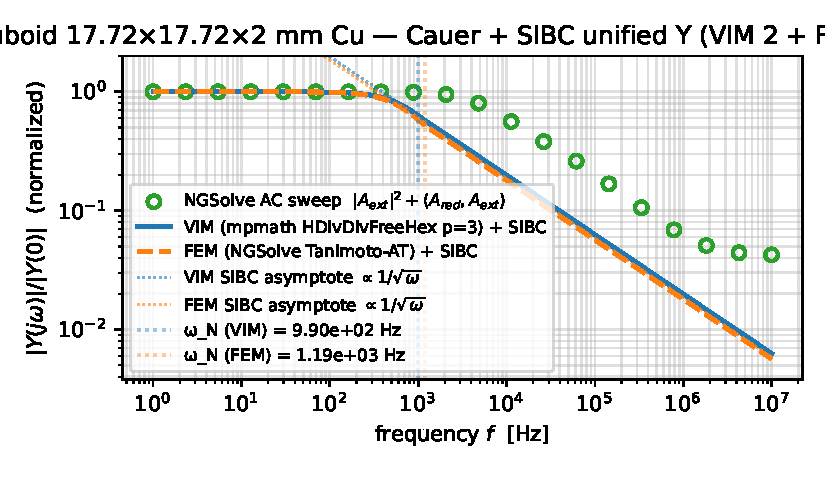
\includegraphics[width=0.98\linewidth]{A1_sibc_3stage_final.pdf}
\vspace{-0.3em}
\caption{Cauer + SIBC unified $|Y(j\omega)|/|Y(0)|$ for the $17.72\!\times\!17.72\!\times\!2$\,mm Cu cuboid in $B_z$.  VIM (solid, two Cauer rungs at $p\!=\!3$, $81$ dof) and NGSolve Tanimoto-AT (dashed, three mesh-converged rungs at $p\!=\!3$, $h\!=\!0.5$\,mm) overlap across nine decades.  Green circles: independent NGSolve AC sweep ground truth -- matches the unified prediction in the Cauer regime and lies slightly below the SIBC seam at high $\omega$ owing to finite-conductor Faraday shielding.}
\label{fig:a1_sibc_compare}
\vspace{-0.8em}
\end{figure}

\begin{thebibliography}{1}
\footnotesize
\bibitem{Kameari_2018} A.~Kameari \emph{et al.}, IEEE Trans.\ Magn.\ {\bf 54}, 3, 2018.
\bibitem{Kuriyama_2019} K.~Kuriyama \emph{et al.}, IEEE Trans.\ Magn.\ {\bf 55}, 6, 2019.
\bibitem{Matsuo_2026} T.~Matsuo, IEEJ SA/RM-26-014, 2026.
\bibitem{Stoll1974} R.~L.~Stoll, {\it The Analysis of Eddy Currents}, Clarendon, 1974.
\bibitem{Wall1948} H.~S.~Wall, {\it Analytic Theory of Continued Fractions}, Van Nostrand, 1948.
\bibitem{Schoberl_Zaglmayr} J.~Sch\"oberl and S.~Zaglmayr, COMPEL {\bf 24}, 374, 2005.
\bibitem{Nagamine_2026} M.~Nagamine \emph{et al.}, submitted, 2026.
\end{thebibliography}

% that's all folks
\end{document}
